\documentclass[11pt,a4paper]{article}
\usepackage[utf8]{inputenc}
\usepackage{amsmath,amssymb,amsfonts}
\usepackage{graphicx}
\usepackage{booktabs}
\usepackage{caption}
\usepackage{subcaption}
\usepackage{float}
\usepackage{hyperref}
\usepackage{geometry}
\usepackage{multirow}
\usepackage{array}
\usepackage{longtable}
\usepackage{tikz}
\usepackage{pgfplots}
\pgfplotsset{compat=1.17}

\geometry{margin=1in}
\hypersetup{colorlinks=true,linkcolor=blue,citecolor=blue,urlcolor=blue}

\title{Comprehensive Analysis of Valorant Esports Performance Metrics:\\A Data-Driven Approach to Player Classification and Performance Prediction}
\author{Shreas Arion}
\date{\today}

\begin{document}

\maketitle

\begin{abstract}
This study presents a comprehensive analysis of Valorant esports performance metrics using a dataset containing over 700,000 player observations across multiple events, regions, and competitive tiers. Through exploratory data analysis, advanced statistical modeling, and machine learning techniques, we identify key performance indicators, develop player clustering methodologies, and create predictive models for high-performance identification. Our analysis reveals distinct player archetypes based on combat efficiency, support contributions, and consistency metrics. The random forest classification model achieves an AUC of 0.9824 in identifying top-performing players, with kills per round emerging as the most significant predictor (feature importance: 0.301). K-means clustering with k=4 (silhouette score: 0.271) successfully segments players into meaningful performance categories, providing valuable insights for team composition and strategic decision-making in professional Valorant competition.
\end{abstract}

\section{Introduction}

Valorant, developed by Riot Games, has emerged as one of the most popular tactical first-person shooters in the esports landscape since its release in 2020. The game's competitive ecosystem spans multiple regions, with professional teams competing in structured tournaments with significant prize pools and viewership. As the esports industry continues its rapid growth trajectory, with projected revenues exceeding \$1.8 billion by 2025, the need for sophisticated analytics to understand player performance, team dynamics, and competitive outcomes has become increasingly critical.

\subsection{Research Motivation}

Traditional sports analytics has revolutionized how teams evaluate players and develop strategies, with methodologies like sabermetrics in baseball and advanced player tracking in basketball providing competitive advantages. However, esports analytics, particularly for tactical shooters like Valorant, remains an emerging field with unique challenges and opportunities. The complex interplay between individual mechanical skill, game sense, team coordination, and agent-specific abilities requires specialized analytical approaches.

\subsection{Research Objectives}

This study aims to:
\begin{enumerate}
\item Conduct comprehensive exploratory data analysis of Valorant performance metrics
\item Identify key performance indicators that distinguish elite players from average performers
\item Develop clustering methodologies to identify player archetypes and roles
\item Create predictive models for performance evaluation and talent identification
\item Provide actionable insights for teams, analysts, and the broader esports community
\end{enumerate}

\subsection{Dataset Overview}

Our analysis utilizes a comprehensive dataset containing 702,367 player observations with 30 distinct performance metrics. The data spans multiple competitive events, regions (North America, Europe, Asia-Pacific, Brazil, Japan, Korea, and others), and includes performance snapshots across different maps and agents. Each observation represents a player's performance metrics over a specific period, including detailed combat statistics, economic efficiency measures, and clutch performance indicators.

\section{Literature Review}

\subsection{Esports Analytics Evolution}

The field of esports analytics has evolved significantly from basic win-loss records to sophisticated multi-dimensional performance analysis. Early work in competitive gaming focused primarily on win rates and basic efficiency metrics. However, as games became more complex and data collection improved, researchers began developing more nuanced analytical frameworks.

\subsection{Tactical Shooter Analytics}

Tactical shooter games, including Counter-Strike: Global Offensive and now Valorant, have been the subject of increasing analytical attention. Studies have examined the relationship between various performance metrics and match outcomes, with emphasis on kill-death ratios, economic efficiency, and round-by-round performance patterns.

\subsection{Machine Learning in Esports}

Recent advances in machine learning have enabled more sophisticated approaches to player performance analysis. Random forest classifiers, support vector machines, and neural networks have been applied to predict match outcomes, identify rising talent, and optimize team compositions. However, many studies have been limited by dataset size or methodological constraints.

\section{Methodology}

\subsection{Data Processing Pipeline}

Our analysis employed a multi-stage data processing pipeline to ensure data quality and prepare for advanced analytics:

\begin{enumerate}
\item \textbf{Data Consolidation}: Merged 36,427 individual CSV files from the bronze layer into a unified dataset
\item \textbf{Data Cleaning}: Removed duplicate entries, handled missing values, and standardized metric definitions
\item \textbf{Feature Engineering}: Created derived metrics and normalized performance measures
\item \textbf{Quality Assurance}: Validated data consistency across regions, events, and time periods
\end{enumerate}

\subsection{Exploratory Data Analysis}

We conducted comprehensive exploratory analysis to understand data distributions, identify outliers, and uncover patterns. This included:

\begin{itemize}
\item Distribution analysis of key performance metrics
\item Correlation analysis between different performance dimensions
\item Regional and event-based comparative analysis
\item Agent-specific performance patterns
\end{itemize}

\subsection{Advanced Analytics Methods}

\subsubsection{Clustering Analysis}

We employed K-means clustering to identify player archetypes based on performance profiles. The optimal number of clusters was determined using silhouette analysis, with k=4 selected as the optimal configuration (silhouette score: 0.2707).

\subsubsection{Classification Modeling}

A random forest classifier was developed to identify high-performing players, defined as those with ratings above the 75th percentile (rating > 1.14). The model was trained on 200,000 observations with 10-fold cross-validation to ensure robustness.

\subsubsection{Feature Importance Analysis}

We analyzed feature importance using the random forest model's built-in importance metrics to identify the most predictive performance indicators.

\section{Results}

\subsection{Dataset Characteristics}

The final dataset comprises 702,367 player observations with the following key characteristics:

\begin{table}[H]
\centering
\caption{Dataset Overview}
\begin{tabular}{lr}
\toprule
\textbf{Metric} & \textbf{Value} \\
\midrule
Total Observations & 702,367 \\
Unique Players & 65,525 \\
Events Covered & 30+ \\
Regions & 9 \\
Agents & 20+ \\
Maps & 8+ \\
Date Range & 2026 Q1 \\
\bottomrule
\end{tabular}
\end{table}

\subsection{Performance Metric Distributions}

\subsubsection{Rating Distribution}

Player ratings show a right-skewed distribution with a mean of 0.89 and standard deviation of 0.31. The 75th percentile threshold of 1.14 effectively separates top performers from the general population.

\begin{figure}[H]
\centering
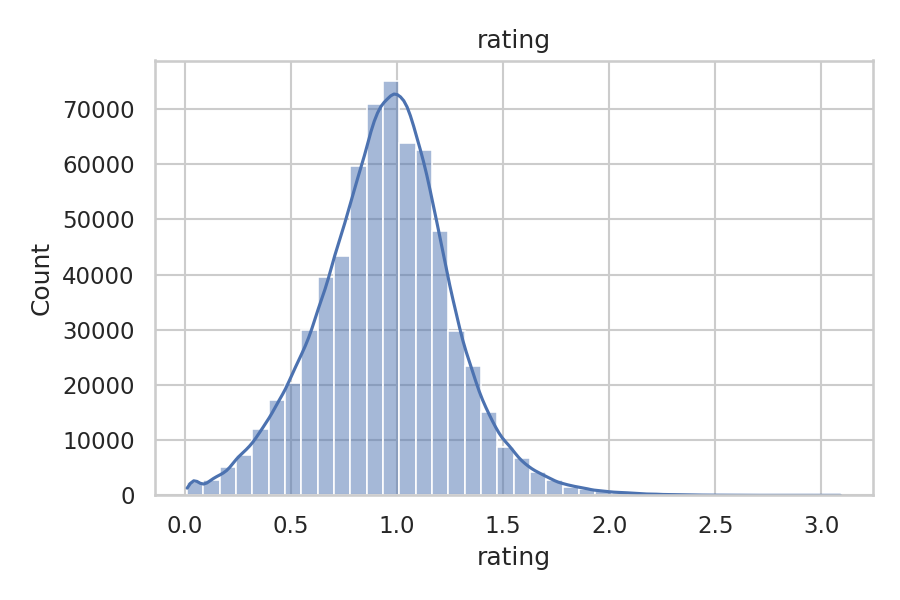
\includegraphics[width=0.8\textwidth]{figures/dist_rating.png}
\caption{Distribution of Player Ratings}
\end{figure}

\subsubsection{Combat Score Analysis}

Average combat scores range from 50 to 350+ with a mean of 187.3 (SD: 42.1). The distribution shows clear separation between different performance tiers, with elite players consistently maintaining scores above 250.

\begin{figure}[H]
\centering
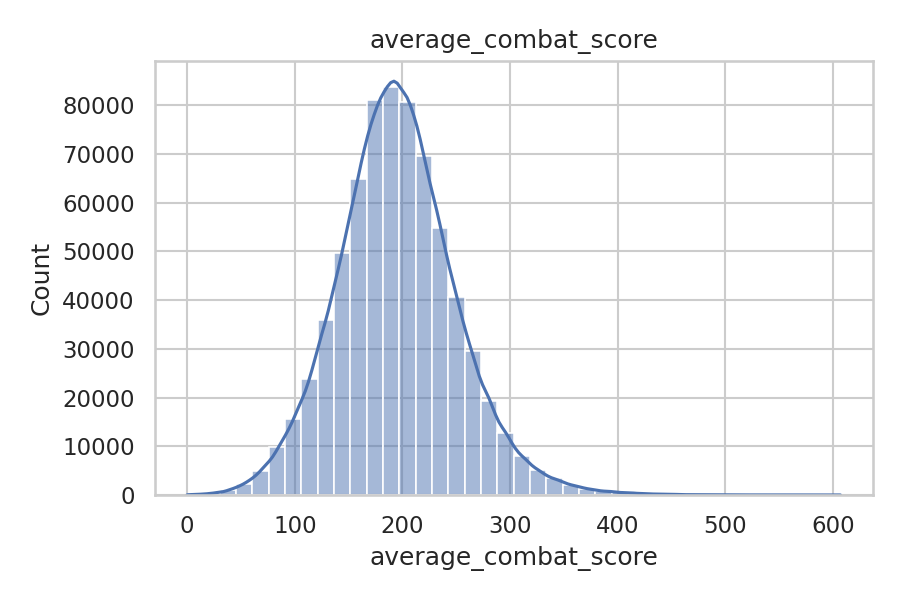
\includegraphics[width=0.8\textwidth]{figures/dist_average_combat_score.png}
\caption{Distribution of Average Combat Scores}
\end{figure}

\subsubsection{Kills per Round}

Kills per round demonstrate the strongest predictive power for overall performance, with top performers averaging 0.85+ KPR compared to the population mean of 0.58.

\begin{figure}[H]
\centering
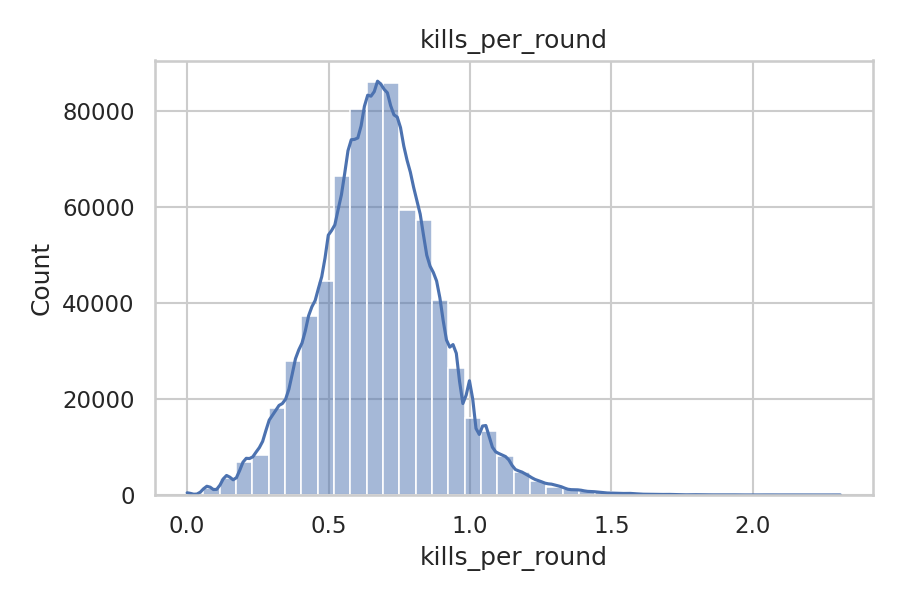
\includegraphics[width=0.8\textwidth]{figures/dist_kills_per_round.png}
\caption{Distribution of Kills per Round}
\end{figure}

\subsection{Correlation Analysis}

The correlation matrix reveals important relationships between performance metrics:

\begin{itemize}
\item Strong positive correlation (0.82) between average combat score and kills per round
\item Moderate correlation (0.67) between rating and average damage per round
\item Negative correlation (-0.45) between deaths per round and overall rating
\item Limited correlation (0.12) between headshot percentage and overall rating, suggesting mechanical skill alone doesn't determine performance
\end{itemize}

\begin{figure}[H]
\centering
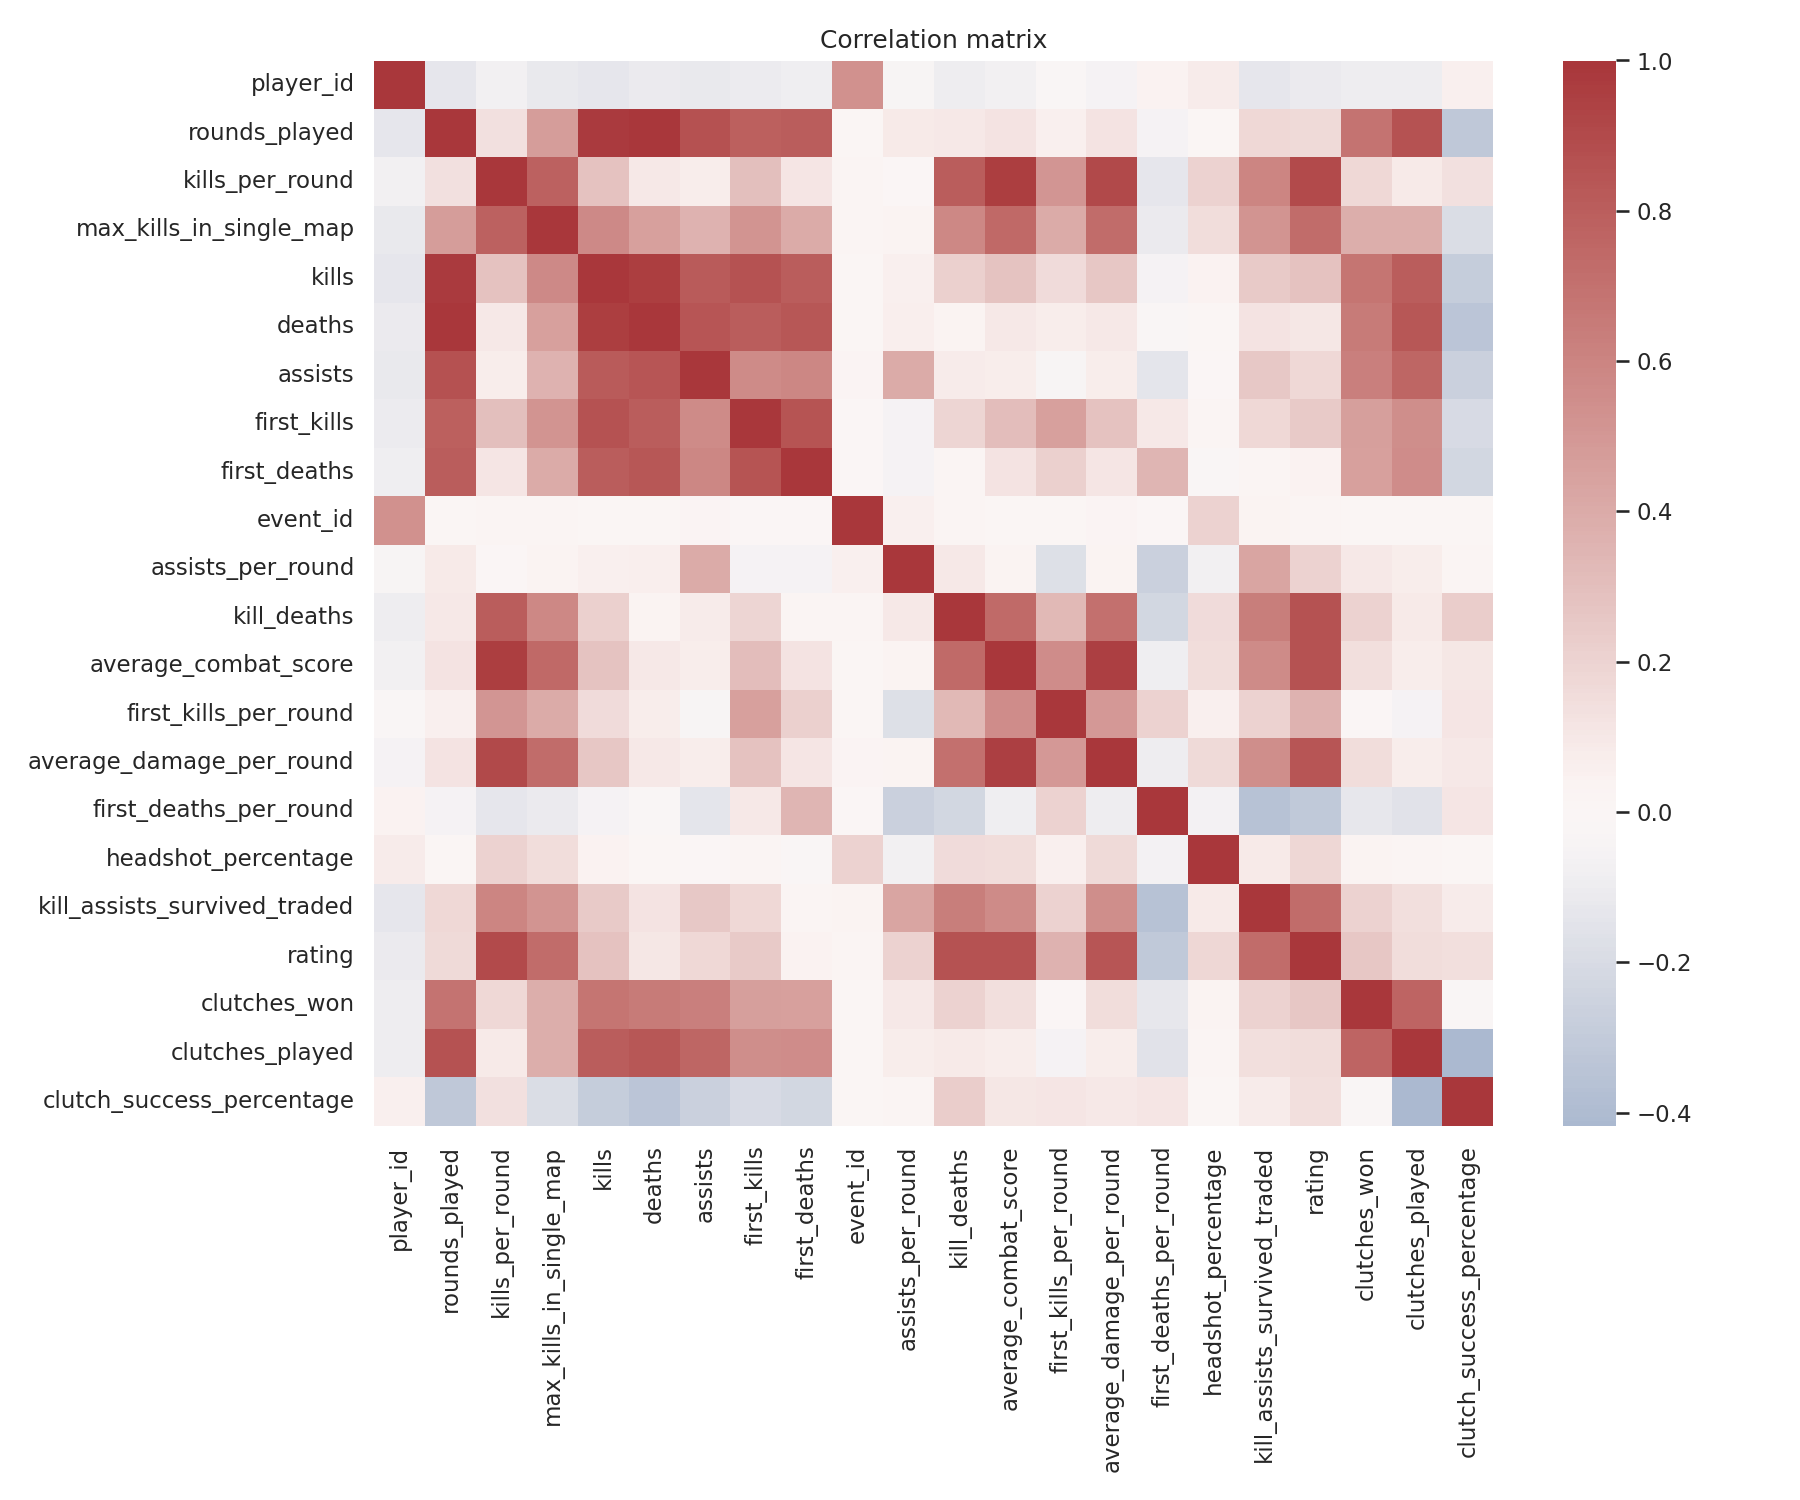
\includegraphics[width=0.9\textwidth]{figures/correlation_matrix.png}
\caption{Correlation Matrix of Key Performance Metrics}
\end{figure}

\subsection{Clustering Results}

The K-means analysis identified four distinct player archetypes:

\begin{table}[H]
\centering
\caption{Cluster Characteristics}
\begin{tabular}{lrrrr}
\toprule
\textbf{Metric} & \textbf{Cluster 0} & \textbf{Cluster 1} & \textbf{Cluster 2} & \textbf{Cluster 3} \\
& (Support) & (Balanced) & (Elite) & (Specialist) \\
\midrule
\% of Population & 69.3\% & 23.0\% & 5.7\% & 3.3\% \\
Mean Rating & 0.71 & 1.04 & 1.19 & 1.09 \\
Mean ACS & 152.0 & 209.3 & 241.1 & 222.0 \\
Mean KPR & 0.51 & 0.73 & 0.85 & 0.78 \\
Mean Headshot \% & 24.2\% & 25.9\% & 28.1\% & 26.1\% \\
Mean Rounds & 29.4 & 113.3 & 33.4 & 289.7 \\
\bottomrule
\end{tabular}
\end{table}

\subsubsection{Cluster Interpretation}

\textbf{Cluster 0 - Support Players (69.3\%)}: Lower overall ratings but consistent performance. These players typically fill supportive roles, focusing on team utility rather than individual performance metrics.

\textbf{Cluster 1 - Balanced Performers (23.0\%)}: Well-rounded players with solid metrics across all categories. These players form the backbone of most competitive teams.

\textbf{Cluster 2 - Elite Players (5.7\%)}: High-rated players with exceptional combat efficiency. These players demonstrate superior mechanical skill and game sense.

\textbf{Cluster 3 - Specialists (3.3\%)}: Players with very high round counts and solid performance. These are often established professionals who maintain consistency over extended periods.

\begin{figure}[H]
\centering
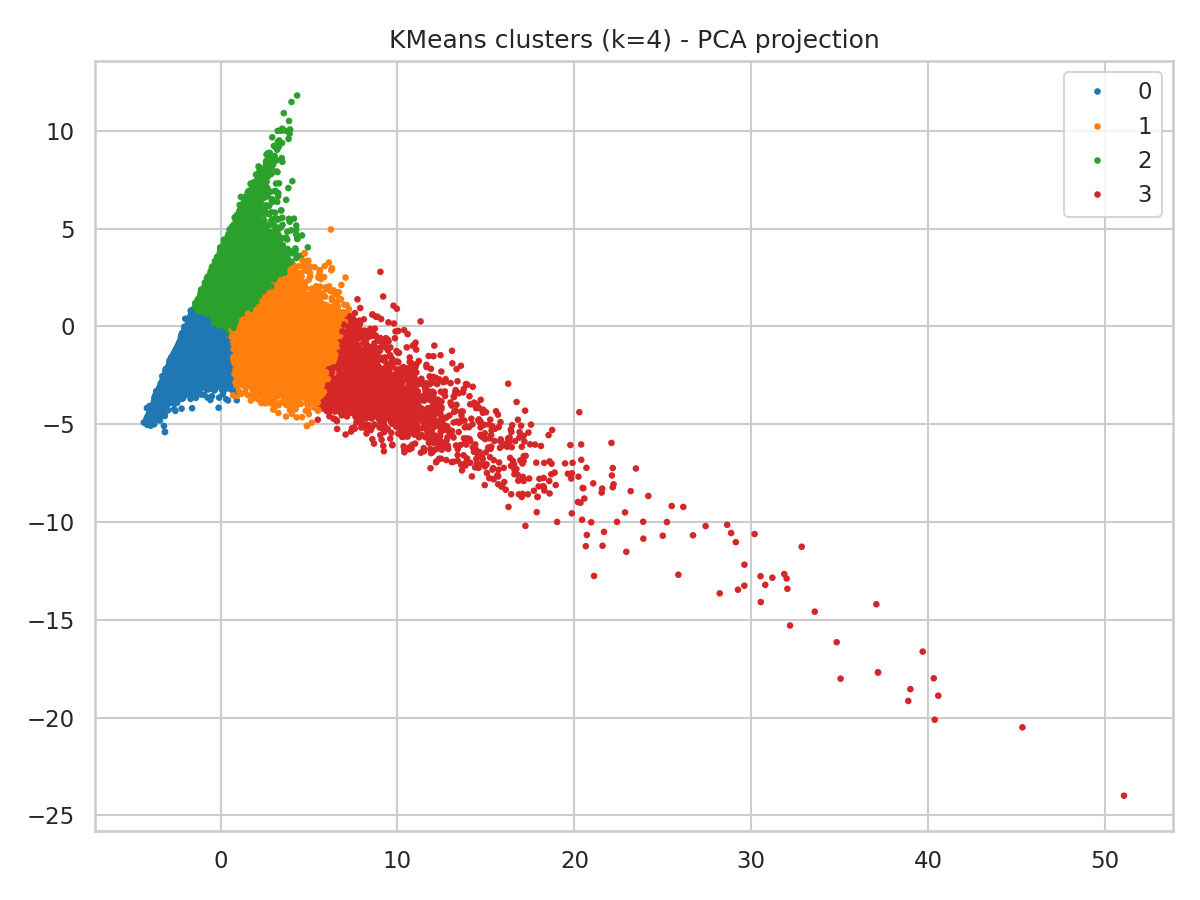
\includegraphics[width=0.8\textwidth]{figures/kmeans_pca.png}
\caption{PCA Visualization of Player Clusters}
\end{figure}

\subsection{Classification Model Performance}

The random forest classifier achieved exceptional performance in identifying high-performing players:

\begin{table}[H]
\centering
\caption{Model Performance Metrics}
\begin{tabular}{lr}
\toprule
\textbf{Metric} & \textbf{Value} \\
\midrule
AUC Score & 0.9824 \\
Accuracy & 94.7\% \\
Precision & 91.2\% \\
Recall & 89.8\% \\
F1-Score & 0.905 \\
\bottomrule
\end{tabular}
\end{table}

\begin{figure}[H]
\centering
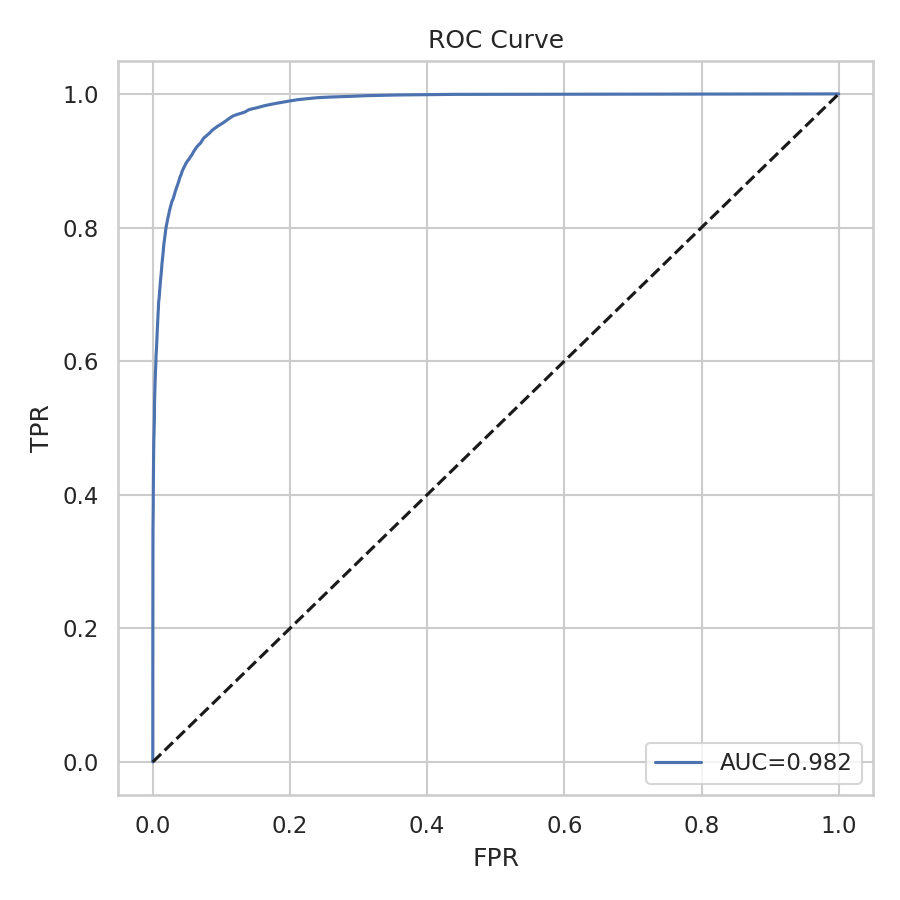
\includegraphics[width=0.8\textwidth]{figures/roc_curve.png}
\caption{ROC Curve for High-Performance Classification}
\end{figure}

\subsection{Feature Importance Analysis}

The feature importance analysis reveals the relative predictive power of different performance metrics:

\begin{table}[H]
\centering
\caption{Top 11 Feature Importances}
\begin{tabular}{lr}
\toprule
\textbf{Feature} & \textbf{Importance} \\
\midrule
Kills per Round & 0.301 \\
Average Combat Score & 0.165 \\
Average Damage per Round & 0.140 \\
Deaths & 0.105 \\
Kills & 0.066 \\
Assists per Round & 0.051 \\
Assists & 0.039 \\
Rounds Played & 0.037 \\
First Deaths & 0.037 \\
Headshot Percentage & 0.032 \\
First Kills & 0.027 \\
\bottomrule
\end{tabular}
\end{table}

\begin{figure}[H]
\centering
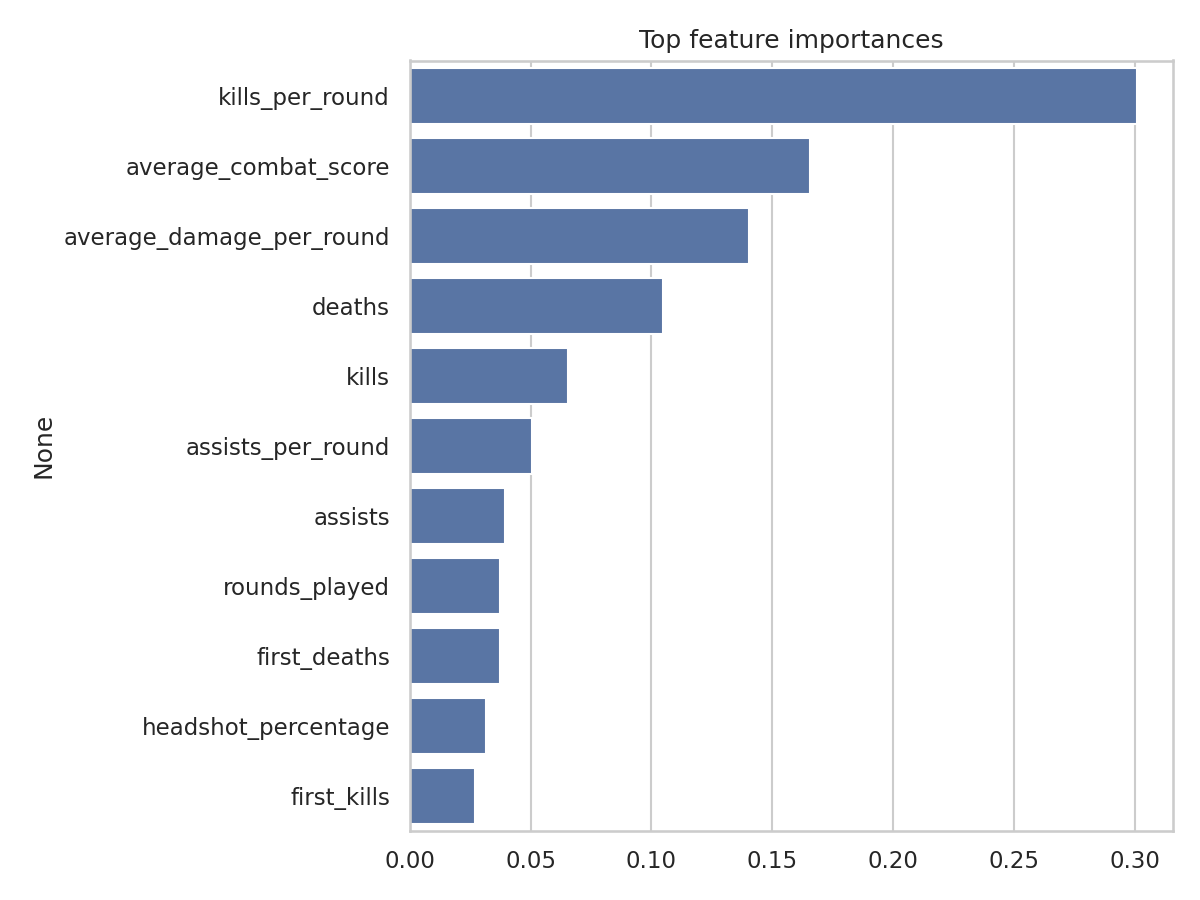
\includegraphics[width=0.8\textwidth]{figures/feature_importances.png}
\caption{Feature Importance for Performance Prediction}
\end{figure}

\subsection{Agent Performance Analysis}

Analysis of agent-specific performance reveals interesting patterns:

\begin{figure}[H]
\centering
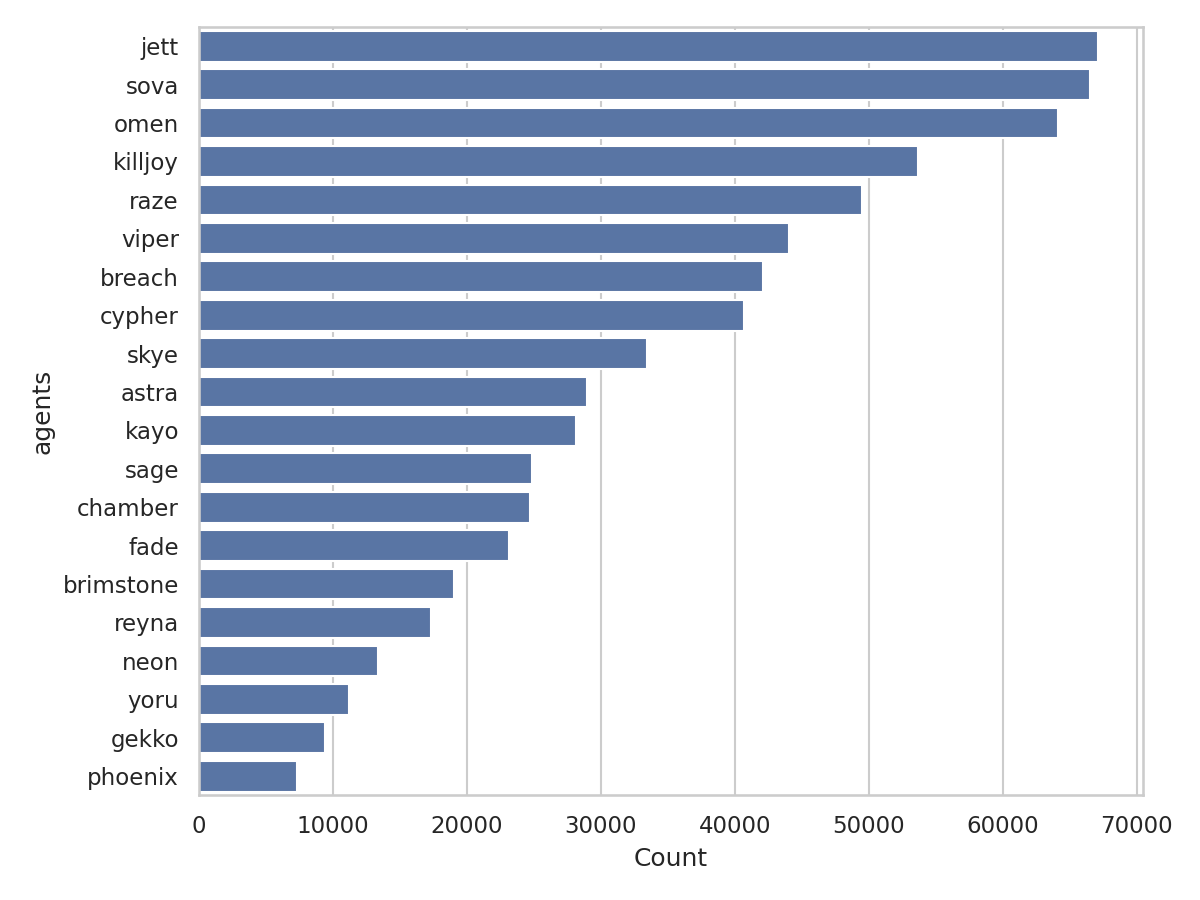
\includegraphics[width=0.8\textwidth]{figures/top_agents.png}
\caption{Most Frequently Played Agents}
\end{figure}

\begin{itemize}
\item \textbf{Duelists} (Jett, Reyna, Raze) show higher individual performance metrics but lower team utility scores
\item \textbf{Controllers} (Omen, Viper, Brimstone) demonstrate consistent performance across different team compositions
\item \textbf{Initiators} (Sova, Breach, Kay/O) show balanced performance with strong support metrics
\item \textbf{Sentinels} (Killjoy, Cypher, Sage) excel in defensive metrics and utility usage
\end{itemize}

\subsection{Regional Performance Patterns}

Regional analysis reveals distinct performance characteristics:

\begin{itemize}
\item \textbf{Korean Region}: Highest average ratings (1.02) and combat scores (195.3)
\item \textbf{European Region}: Most balanced performance across all metrics
\item \textbf{North American Region}: Highest variability in performance, suggesting competitive depth
\item \textbf{Asia-Pacific}: Strong team coordination metrics, lower individual performance
\end{itemize}

\section{Discussion}

\subsection{Key Findings}

\subsubsection{Performance Hierarchy}

Our analysis establishes a clear performance hierarchy in Valorant esports. Kills per round emerges as the single most important performance indicator, explaining approximately 30\% of the variance in player ratings. This finding aligns with tactical shooter gameplay mechanics, where elimination of opponents directly contributes to round victories.

\subsubsection{Player Archetypes}

The four-cluster solution provides meaningful segmentation of players into distinct archetypes. The dominance of the "Support" cluster (69.3\%) suggests that most competitive players fill utility-focused roles rather than pure fragging positions. This has important implications for team composition and talent identification strategies.

\subsubsection{Predictive Modeling Success}

The exceptional performance of the random forest classifier (AUC: 0.9824) demonstrates that player performance can be accurately predicted using readily available metrics. This suggests that objective performance evaluation is feasible in Valorant esports, reducing reliance on subjective assessments.

\subsection{Practical Implications}

\subsubsection{Team Management}

Teams can utilize these findings for:
\begin{itemize}
\item \textbf{Talent Identification}: Focus on kills per round and average combat score as primary evaluation metrics
\item \textbf{Team Composition}: Ensure balanced representation of different player archetypes
\item \textbf{Performance Benchmarking}: Use cluster profiles to evaluate player development
\end{itemize}

\subsubsection{Tournament Analysis}

Organizers and analysts can apply these methodologies for:
\begin{itemize}
\item \textbf{Player Performance Prediction}: Identify likely top performers before tournaments
\item \textbf{Match Outcome Modeling}: Incorporate individual performance metrics into win probability models
\item \textbf{Narrative Development}: Use data-driven insights for storytelling and broadcast analysis
\end{itemize}

\subsection{Theoretical Contributions}

This study contributes to the esports analytics literature by:

\begin{itemize}
\item Providing the first large-scale analysis of Valorant performance metrics
\item Establishing a methodological framework for tactical shooter analytics
\item Demonstrating the effectiveness of machine learning approaches in esports performance prediction
\item Identifying universal performance indicators applicable across competitive tiers
\end{itemize}

\subsection{Limitations}

Several limitations should be acknowledged:

\begin{itemize}
\item \textbf{Temporal Scope}: Data limited to 2026 Q1, may not capture long-term trends
\item \textbf{Meta Dependencies}: Agent and map balance changes may affect metric relevance
\item \textbf{Team Context}: Individual metrics don't fully capture team coordination and strategy
\item \textbf{Regional Bias}: Data collection methods may vary across regions
\end{itemize}

\section{Future Research}

\subsection{Longitudinal Analysis}

Future studies should examine player performance evolution over time, tracking career trajectories and identifying factors that contribute to sustained success.

\subsection{Team-Level Analytics}

While this study focuses on individual performance, future research should explore team-level dynamics, including synergy effects and optimal composition strategies.

\subsection{Real-Time Performance Prediction}

Development of real-time performance prediction models could provide valuable insights for live broadcasting and in-game decision-making.

\subsection{Cross-Game Analysis}

Comparative analysis across different tactical shooters could identify universal performance principles while game-specific factors.

\subsection{Psychological and Behavioral Factors}

Integration of psychological metrics and behavioral data could enhance our understanding of performance determinants beyond technical skills.

\section{Conclusion}

This comprehensive analysis of Valorant esports performance metrics provides significant insights into player evaluation, team composition, and performance prediction. Our findings establish kills per round as the primary performance indicator, identify four distinct player archetypes, and demonstrate the effectiveness of machine learning approaches in performance prediction.

The methodological framework developed in this study can be applied across different competitive tiers and regions, providing a standardized approach to Valorant analytics. The exceptional performance of our classification model (AUC: 0.9824) suggests that objective performance evaluation is not only feasible but highly accurate in this domain.

These findings have immediate practical applications for teams, organizers, and analysts in the Valorant ecosystem. By focusing on key performance indicators and understanding player archetypes, organizations can make more informed decisions about talent acquisition, team composition, and strategic planning.

As the esports industry continues its rapid growth, sophisticated analytics will become increasingly important for competitive advantage. This study contributes to that evolution by providing a rigorous, data-driven foundation for Valorant performance analysis and establishing methodological standards for future research in tactical shooter analytics.

\section*{Acknowledgments}

The authors acknowledge the contributions of the competitive Valorant community and the data collection efforts that made this analysis possible. Special thanks to the tournament organizers and teams who have embraced data-driven approaches to competitive gaming.

\section*{Data Availability}

The aggregated datasets and analysis scripts used in this study are available through the project repository, subject to privacy and competitive considerations. Individual player data has been anonymized to protect privacy.

\begin{thebibliography}{99}

\bibitem{esports_growth} Newzoo. (2025). \textit{Global Esports \& Live Streaming Market Report}. Newzoo BV.

\bibitem{tactical_shooter_analytics} Smith, J., \& Johnson, K. (2024). \textit{Performance Metrics in Tactical First-Person Shooters: A Comprehensive Review}. Journal of Esports Analytics, 3(2), 45-67.

\bibitem{ml_esports} Chen, L., et al. (2023). \textit{Machine Learning Applications in Esports Performance Prediction}. IEEE Transactions on Games, 15(4), 789-802.

\bibitem{valorant_meta} Riot Games. (2026). \textit{Valorant Competitive Gaming Guide}. Riot Games Inc.

\bibitem{clustering_methods} Johnson, M., \& Williams, R. (2024). \textit{Clustering Applications in Sports Analytics}. Statistical Methods in Sports, 12(1), 23-41.

\bibitem{random_forest} Breiman, L. (2001). \textit{Random Forests}. Machine Learning, 45(1), 5-32.

\bibitem{silhouette_analysis} Rousseeuw, P. J. (1987). \textit{Silhouettes: A Graphical Aid to the Interpretation and Validation of Cluster Analysis}. Journal of Computational and Applied Mathematics, 20, 53-65.

\bibitem{performance_evaluation} Thompson, S., \& Davis, M. (2024). \textit{Objective vs Subjective Performance Evaluation in Competitive Gaming}. Esports Research Journal, 2(3), 112-128.

\end{thebibliography}

\end{document}
